\textbf{COLUNI 2025 -- Questão 34}\par\medskip A cadeia produtiva do café está solidamente estabelecida no território do Brasil e movimenta vários tipos de atividades a ela vinculadas. Observe a seguir os mapas que representam algumas das atividades econômicas relacionadas à produção cafeeira brasileira.

\begin{center}
\begin{minipage}[t]{0.48\linewidth}\centering
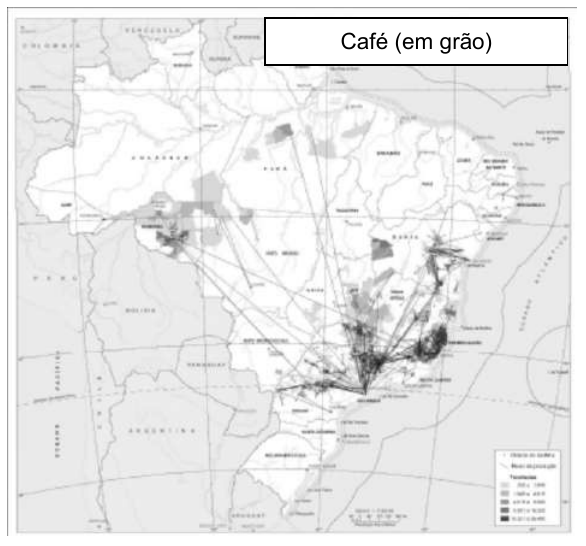
\includegraphics[width=\linewidth]{static/simulados/coluni/figuras/2025/questao-34/figura-1.png}
\end{minipage}\hfill\begin{minipage}[t]{0.48\linewidth}\centering
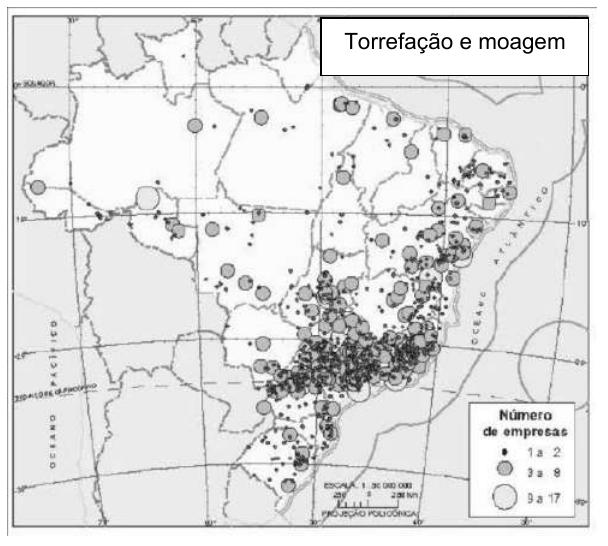
\includegraphics[width=\linewidth]{static/simulados/coluni/figuras/2025/questao-34/figura-2.png}
\end{minipage}

\vspace{0.5em}

\begin{minipage}[t]{0.48\linewidth}\centering
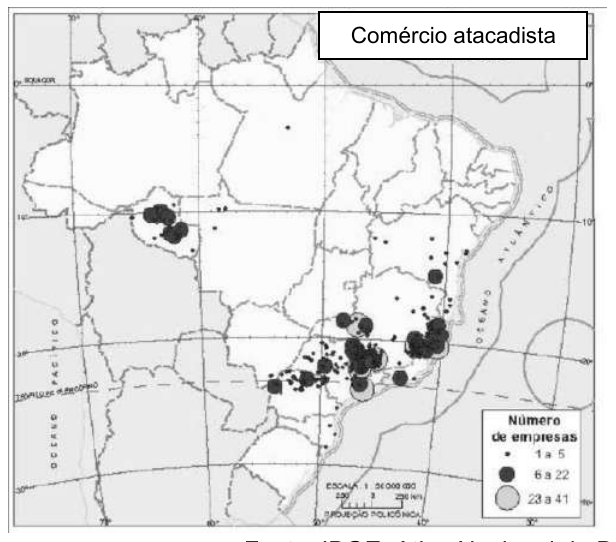
\includegraphics[width=\linewidth]{static/simulados/coluni/figuras/2025/questao-34/figura-3.png}
\end{minipage}\hfill\begin{minipage}[t]{0.48\linewidth}\centering
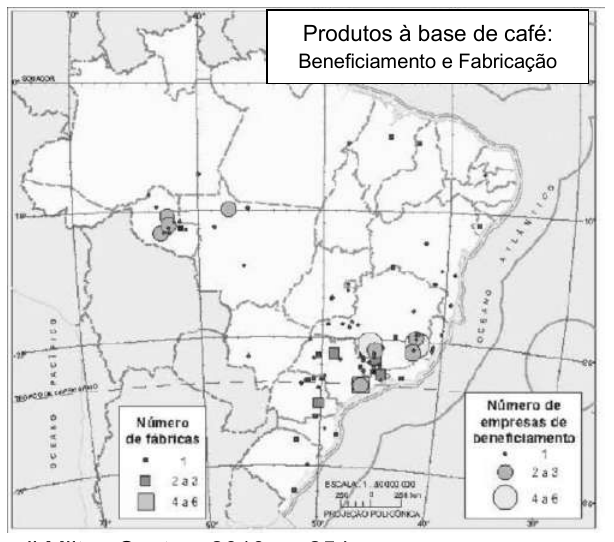
\includegraphics[width=\linewidth]{static/simulados/coluni/figuras/2025/questao-34/figura-4.png}
\end{minipage}
\end{center}

\begin{center}Fonte: IBGE, Atlas Nacional do Brasil Milton Santos, 2010, p. 254.\end{center}

A respeito da distribuição das atividades vinculadas à produção cafeeira no território brasileiro, assinale a afirmativa CORRETA:
\begin{enumerate}
\item A produção cafeeira está uniformemente distribuída pelo território.
\item A torrefação e a moagem possuem maior representatividade na região Nordeste.
\item Os produtos à base de café apresentam distribuição semelhante a do comércio atacadista.
\item O escoamento da produção cafeeira se beneficia da eficiente rede de transporte fluvial e marítimo.
\end{enumerate}
